%%%%%thesis preamble starts below%%%%%%%%%%%%%
%%%%%%%%%%%%%%%%%%%%%%%%%%%%%%%%%%%%%%%%%%%%%%%%%%%%
% Document type, global settings, and packages
%%%%%%%%%%%%%%%%%%%%%%%%%%%%%%%%%%%%%%%%%%%%%%%%%%%%
%\documentclass[12pt,notitlepage]{article}
\documentclass[12pt]{article}
%\documentclass[12pt]{report}   %12 point font for Times New Roman
\usepackage{graphicx}  %for images and plots
\usepackage[letterpaper, left=1.5in, right=1in, top=1in, bottom=1in]{geometry}
\usepackage[doublespacing]{setspace}  %use this package to set linespacing as desired
\usepackage{times}  %set Times New Roman as the font
\usepackage[explicit]{titlesec}  %title control and formatting
\usepackage[titles]{tocloft}  %table of contents control and formatting
%%\usepackage[backend=bibtex, sorting=none]{biblatex}  %reference manager
\usepackage{natbib}
\usepackage[bookmarks=true, hidelinks]{hyperref}
\usepackage[page]{appendix}  %for appendices
\usepackage{rotating}  %for rotated, landscape images
\usepackage{pdfpages} %%for including an existing pdf in the newly generated pdf; here, I am including my annotation guidelines as an appendix
\usepackage{multirow}
\usepackage{gb4e} % MD: some versions of latex need this package to be loaded last
\noautomath %%LK: I found that adding this immediately after gb4e fixes the problem!
%%%%%%LK: Below: I added from BEA2013
\usepackage{rotating}
\usepackage{tikz}
\usetikzlibrary{shapes,arrows}
\usepackage{graphicx}
\usepackage{tikz-dependency}
\usepackage{natbib}
\usepackage{url}
%\usepackage{gb4e} % MD: some versions of latex need this package to be loaded last
\usepackage{amsmath}
\DeclareMathOperator*{\argmax}{arg\,max}
\DeclareMathOperator*{\argmin}{arg\,min}
\usepackage{tikz-qtree}
\usepackage{multirow}
\usepackage{rotating}
\usepackage{booktabs}
%%%%%%LK: Above: I added from BEA2013
\usepackage{array}
\newcommand{\PreserveBackslash}[1]{\let\temp=\\#1\let\\=\temp}
\newcolumntype{C}[1]{>{\PreserveBackslash\centering}p{#1}}
\newcolumntype{R}[1]{>{\PreserveBackslash\raggedleft}p{#1}}
\newcolumntype{L}[1]{>{\PreserveBackslash\raggedright}p{#1}}

%%%%%%%%%%%%%%%%%%%%%%%%%%%%%%%%%%%%%%%%%%
%Below copied from naaclhlt2018.sty
%%%%%%%%%%%%%%%%%%%%%%%%%%%%%%%%%%%%%%%%%%
%\RequirePackage{natbib}
% for citation commands in the .tex, authors can use:
% \citep, \citet, and \citeyearpar for compatibility with natbib, or
% \cite, \newcite, and \shortcite for compatibility with older ACL .sty files
\renewcommand\cite{\citep}	% to get "(Author Year)" with natbib    
\newcommand\shortcite{\citeyearpar}% to get "(Year)" with natbib    
\newcommand\newcite{\citet}	% to get "Author (Year)" with natbib    
%%%%%%%%%%%%%%%%%%%%%%%%%%%%%%%%%%%%%%%%%%
%Above copied from naaclhlt2018.sty
%%%%%%%%%%%%%%%%%%%%%%%%%%%%%%%%%%%%%%%%%%
\newcommand{\feat}[1]{\textsc{#1}}
\newcommand{\param}[1]{\texttt{#1}}
\newcommand{\md}[1]{\marginpar{\scriptsize MD: #1}}
\newcommand{\lk}[1]{\marginpar{\scriptsize LK: #1}}
% for removing all marginpars ==> good for final submission! %%nice trick!
%\renewcommand{\marginpar}[1]{}


\newcommand\BibTeX{B{\sc ib}\TeX}
%%\usepackage{gb4e}  % MD: some versions of latex need this package to be loaded last
%%%%%thesis preamble ends above%%%%%%%%%%%%%




%
%%%%%%annotation guide preamble starts below%%%%%%%%%%%%%
%\documentclass[12pt,notitlepage]{article}
%\usepackage[margin=1in]{geometry}                % See geometry.pdf to learn the layout options. There are lots.
%\geometry{letterpaper}                   % ... or a4paper or a5paper or ... 
%\usepackage{parskip}
%\usepackage{graphicx}
%\usepackage{lipsum}
%\usepackage{natbib}
%\usepackage{url}
%\usepackage{color,soul}
%\usepackage{fancyhdr}
%\usepackage{multirow}
%\usepackage{titlesec}
%\usepackage[linktoc=all]{hyperref}
%\hypersetup{
%    colorlinks,
%    citecolor=black,
%    filecolor=black,
%    linkcolor=black,
%    urlcolor=black
%}
%%
%\newcommand{\feat}[1]{\texttt{#1}}
%\newcommand{\lk}[1]{\marginpar{\linespread{1}\scriptsize LK: #1}}
%\setlength{\parindent}{0pt} %Paragraphs will not be indented
%\linespread{1.3}
%\titleformat{\paragraph}[hang]{\normalfont\normalsize\bfseries}{\theparagraph}{1em}{}

\setcounter{secnumdepth}{4}
\setcounter{tocdepth}{4}
\usepackage{gb4e} % MD: some versions of latex need this package to be loaded last

%
\title{\large{Semantic Analysis of Image-Based Learner Sentences (SAILS)} \\ Annotation Guide \\ Version 1.0, December 19, 2017}
%
\date{}
%%%%%%annotation guide preamble ends above%%%%%%%%%%%%%



\begin{document}
\maketitle
\tableofcontents
\clearpage

\section{Task Background} \label{sec:background}

\subsection{Overview}
In order to best annotate the data, annotators should have a basic understanding of the task used to collect it. The task is a \textbf{picture description task (PDT)}, implemented as an online survey. The PDT consists of 30 items. An \textbf{item} is one image and corresponding question. Each item is displayed on a single page of the online survey, and participants type a response into the provided field before clicking ahead to the next page. The task was conducted with default web browser settings, so browser-based spelling correction tools were available to participants.

The images used are simple digital drawings. No two images are related, and nothing appears in more than one image. Each image was chosen or created to depict a single event or action. In order to focus attention on the main action, images contain very little background or other detail. Participants were instructed to provide one complete sentence capturing the main action in the image. 

The data collected in the task will be used to analyze the differences in English \textbf{native speaker (NS)} and \textbf{non-native speaker (NNS)} language use. The researchers intend to study the many ways in which responses vary, and to compare these variations for NS and NNS responses. Ultimately, the researchers intend to use the NS responses to derive a kind of answer key or \textbf{gold standard (GS)}, which can be used to automatically evaluate the content of NNS responses.

\subsection{Participants}
The following section describes the different participant groups. It is provided for informational purposes only. While annotating, annotators do not need and are not given any information about the source of the responses.

\subsubsection{Non-native speakers}
NNS participants were recruited from intermediate and advanced level English as a Second Language (ESL) courses in the English Language Improvement Program at Indiana University. Roughly 140 NNS students completed the PDT. These participants all performed the task independently in a computer lab, with the researchers present. Responses from this group appear to be given in good faith.

\subsubsection{Native speakers}
Two different groups of NSs participated: familiar NSs and crowd-sourced NSs. All NSs performed the task remotely, without the researchers present.

\paragraph{Familiar NSs}
40 \textbf{familiar} NS participants completed the full task. They were recruited among friends, family and acquaintances of the researchers. Responses from this group appear to be given in good faith.

\paragraph{Crowd-sourced NSs}
Responses were also collected from roughly 330 different \textbf{crowd-sourced} NSs through the online platform, Survey Monkey. The researchers purchased survey responses from the platform's pool of users, who may win prizes or earn donations for charities in exchange for completing surveys. These participants all performed the task remotely, without the researchers present.

Crowd-sourced participants are less likely to complete a lengthy task, so the PDT was divided into four smaller tasks, and each crowd-sourced NS completed only one of these. Additionally, a sizable number of these participants completed only part of their task before abandoning it. The resulting data set is equivalent in size to roughly 150 completed familiar NS PDTs. Responses from the crowd-sourced group are of varying reliability; the majority are legitimate and in good faith, but some responses clearly are not. Some crowd-sourced NSs simply typed random characters in the response fields in order to move on to the next item and complete the task with minimal time and effort. Others responded with jokes, sarcasm or profanity.

\subsection{Instructions} 
Before beginning the task, respondents read a short page of instructions including an example item and possible responses. The instructions are as follows:

\begin{quotation}\noindent
In this task, you will view a set of images. For each image, please write \textbf{one sentence} to answer the question provided with the image. It is important to answer with a \textbf{complete sentence}, not a word or phrase.
\end{quotation}

English native speakers (NSs) and non-native speakers (NNSs) complete slightly different versions of the task. The items are identical in both versions, but whereas NNSs provide one response to each question, in the NS version, respondents are asked to provide two responses to each question. They are given the following additional instructions:

\begin{quotation}\noindent
Then, you will be asked to write a second, \textit{different} answer, which is also a complete sentence. This might involve rewording or reorganizing your first sentence. It does not need to be \textit{completely} different; some words may be the same. If you cannot think of another way to answer the question, you may leave the second answer space empty, but any second responses you provide will be greatly appreciated.
\end{quotation}

\subsection{Item Examples (Targeted and Untargeted)}

The first half of the task consists of 15 \textbf{targeted} items, and the second half consists of 15 \textbf{untargeted} items. Targeted and untargeted items differ only in the question. All targeted items take the form of \textit{What is X doing?}, where \textit{X} varies but is specified in the question, always as the subject (e.g., \textit{the girl}, \textit{the bird}) of the main action in the image. For all untargeted items, the question is always the same: \textit{What is happening?}.

For each image used in the task, a roughly equivalent number of targeted and untargeted responses were collected. Multiple versions of the task were administered; a given image is used in the targeted section for some versions, and in the untargeted section for other versions. In all versions, the targeted items precede the untargeted items. This ordering is intended to avoid the possibility that a participant encounters the question \textit{What is happening?} consistently in the initial items, assumes that this question applies to the entire task, and responds to the later targeted items without reading the questions.

The terms \textit{targeted} and \textit{untargeted} are never used in the task, and participants are not explicitly informed of these differences. They are, however, provided with an example of each type immediately following the instructions, as seen in Figures~\ref{fig:instructions1} and~\ref{fig:instructions2} below.

\begin{figure}[!htb]
\begin{center}
\begin{tabular}{|p{0.7\columnwidth}|}
\hline
\multicolumn{1}{|c|}{\textbf{Example 1}}\\
\hline
\multicolumn{1}{|c|}{
\includegraphics[width=0.4\columnwidth,trim=0 0 0 -3]{figures/ex02.jpg}}\\
\hline
\textbf{\textit{What is the man doing?}}\\
\hline
\textbf{Your sentence:} \\
\textit{The man is shouting.}\\
\hline
\textbf{Your second sentence:} \\
\textit{He is yelling.} \\
\hline
\textbf{There is not a single correct response. Many responses may be possible. Other responses might be:} \\
\textit{The man is yelling something.} \\
\textit{He is speaking loudly.} \\
\hline
\end{tabular}
\end{center}
\caption{An example \textit{targeted} item, as presented in the task instructions. The ``second sentence'' portion is presented to native speakers only.}
\label{fig:instructions1}
\end{figure}


\begin{figure}[!htb]
\begin{center}
\begin{tabular}{|p{0.7\columnwidth}|}
\hline
\multicolumn{1}{|c|}{\textbf{Example 2}}\\
\hline
\multicolumn{1}{|c|}{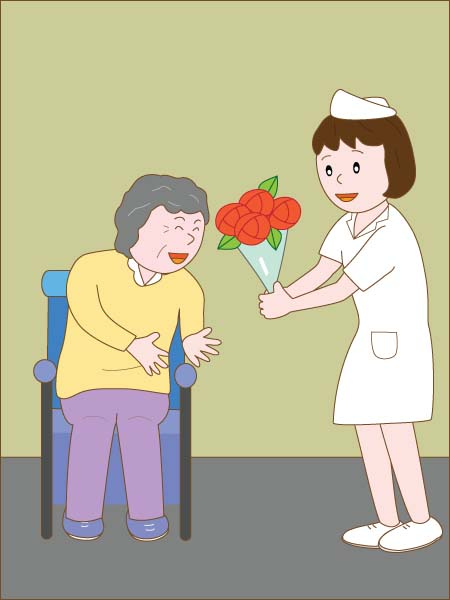
\includegraphics[width=0.4\columnwidth,trim=0 0 0 -3]{figures/ex01.jpg}}\\
\hline
\textbf{\textit{What is happening?}}\\
\hline
\textbf{Your sentence:} \\
\textit{The nurse is giving a patient roses.}\\
\hline
\textbf{Your second sentence:} \\
\textit{A woman is getting flowers from a nurse.} \\
\hline
\textbf{There is not a single correct response. Many responses may be possible. Other responses might be:} \\
\textit{The nurse is giving a lady some red flowers.} \\
\textit{A patient is receiving flowers from a nurse.} \\
\hline
\end{tabular}
\end{center}
\caption{An example \textit{untargeted} item, as presented in the task instructions. The ``second sentence'' portion is presented to native speakers only.}
\label{fig:instructions2}
\end{figure}

\clearpage
\section{Annotating Features}

Each response is annotated according to five dimensions, or \textit{features}. These features, explained below, are referred to as \textit{\textbf{core event, verifiability, answerhood, interpretability}} and \textit{\textbf{grammaticality}}. Annotations for each feature have only two possible values, \textit{yes} or \textit{no} (or \textit{1} or \textit{0}). The annotation for each response is thus an ordered list (i.e., a vector) of zeros and ones. For example, [1, 1, 1, 1, 0] would represent a response that was annotated \textit{no} for grammaticality and \textit{yes} for all other features.

\subsection{Core event} \label{subsec:core-event}
The core event feature primarily considers the following question: \textit{Exactly as written, does the response capture the core event of the item?}

\subsubsection{Contextuality of core event} Annotation for the core event feature is contextual; it must consider the image and question presented in the item. 

\subsubsection{Defining \feat{core event}}
Each image depicts a single \feat{core event} that could be captured by a simple sentence or verb phrase. Each core event involves an action; responses that merely describe a state or feature of the image do not capture the core event. Considering Figure~\ref{fig:dance}, for example, the response \textit{He is a dancing machine} does not capture the core event; it describes a characteristic of the boy, but does not describe what is actually taking place in the image.

\paragraph{Subjects} \label{para:core-event-subjects} The form of a core event is generally similar to that of a \textit{predicate} in traditional grammar. The core event describes what the subject (or agent) is doing. Thus, when annotating for core event, the predicate of the sentence is the most important consideration. However, there are some rules pertaining to the subject. The sentence must include a subject. In the case of targeted items, the subject may be omitted if it can be understood from the question. Annotators should be quite flexible with regard to the subject, with a few restrictions. Even for targeted items, the subject in the response does not need to be identical to the subject provided in the question. For example, in response to \textit{What is the boy doing?}, responses that restate the subject as \textit{guy} or \textit{kid} or proper names like \textit{Peter} should be accepted. Much flexibility with regard to age should be given as well; infants aside, \textit{man}/\textit{boy} should be treated interchangeably, as should \textit{woman}/\textit{girl}. Crucially, the meaning of the subject in the response should not be in conflict with what is shown in the image. Thus, a response that restates the male subject as female or assigns an exclusively female name should not be accepted. More flexibility is allowed for number; a response that depicts a singular subject as plural or vice versa is still acceptable. The rationale for this decision is that the core event feature should avoid penalizing responses for concerns covered by other features. Concerns about number would primarily be covered with the grammaticality and verifiability features. Moreover, while a subject is necessary to fulfill the core event, the focus of this feature is the event itself. In short, responses that assign an incorrect number to the subject  are acceptable, but those that change a subject's gender are not.

\paragraph{Verb forms}
The core event is best fulfilled with a present progressive verb form, but responses that use other verb forms may be acceptable. Crucially, the response should allow for an interpretation in which the verb refers to the specific event displayed in the image. For example, in most contexts, \textit{He enjoys dancing to music} would be interpreted to mean that \textit{in general}, the subject enjoys the activity of dancing to music. However, in this context, it could refer to the event displayed in the image; the sentence could be intended as a narration of the image. Likewise, responses that describe the event in past or future terms might be acceptable; annotatos should use their own best judgment. Responses that use modality or hedging (e.g., \textit{He must be dancing}; \textit{I think he's dancing}), and those that are formed as questions (e.g., \textit{Is he dancing?}) are also acceptable, as long as the core event is present and clearly tied to the appropriate subject (or agent).

\begin{figure}[htb!]
\begin{center}
\begin{tabular}{|l|}
\hline

\includegraphics[width=0.4\columnwidth,trim=0 0 0 -3]{figures/I02.jpg}\\
\hline
1: He's eating a delicious slice of pizza. \\
\hline
2: He's eating pizza, yuck. \\
\hline
3: He will get fat eating pizza. \\
\hline
\end{tabular}
\end{center}
\caption{Item 2 (targeted: \textit{What is the boy doing?}) and example responses.}
\label{fig:eat-pizza}
\end{figure}

\paragraph{Content}
Core events are not predefined; annotators should decide what each core event is and whether or not a response captures it. Moreover, a core event should be conceived of abstractly rather than as a particular phrase or expression. Two responses that convey the same concept in different forms should be judged as equally acceptable. For example, \textit{The man is shouting} and \textit{He is yelling}, as seen in Figure~\ref{fig:instructions1}, convey the same core event using different words.

Given the simplicity of the images, the core event should be clear for each. None of the images depicts any background events that are unrelated to the core event. Any non-core event that could be described either supports the core event or is a cause or effect of the core event. In Figure~\ref{fig:instructions2}, for example, the untargeted question (\textit{What is happening?}) could be answered with \textit{The patient is smiling}, but this is clearly an effect of the core event, in which a nurse is giving the patient flowers. Thus, \textit{The patient is smiling} should be annotated \textit{no} here.

\subsubsection{Alternative interpretations \& inaccurate information} Although every effort was made to produce unambiguous PDT images, reasonable alternative interpretations are seen among the responses for a very small number of items. For example, Figure~\ref{fig:deliver-package} shows a woman seated behind a desk and a man holding a package in front of the desk. Most participants interpret the scene as the man delivering a package to the woman. However, a small number of participants interpret this scene as a man picking up a package from the woman -- a reasonable alternative. Such reasonable alternatives should be annotated \textit{yes} for core event. An even smaller number of participants describe the scene as a student giving a gift to his teacher. However, the ``student'' here is wearing a work uniform and holding a brown parcel with a visible shipping label, so this interpretation should be rejected. Annotators should use their own in judgement in annotating responses that contain variations in interpretation.

As long as the core event is present and linked to a reasonable subject (or agent), inaccurate information in a response should be ignored and the response should be accepted. For Figure~\ref{fig:dance}, for example, \textit{A boy is dancing at a birthday party} should be annotated \textit{yes}. Although we see no evidence of a party, the response nonetheless covers the core event, which is \textit{(boy) is dancing} or something equivalent. Likewise, the (hypothetical) response \textit{The guy is dancing on the moon} should be accepted, because the core event and a reasonable subject are present.

\subsubsection{Language problems} Grammatical and spelling problems do not automatically result in a \textit{no} for the core event feature. Responses with errors that do not obscure the core event may still be annotated as \textit{yes}. In other words, if, despite a language problem, the necessary elements of the core event are intact and their relationship is reasonably interpretable, the response is annotated \textit{yes}. Such cases are typically very minor errors. For Figure~\ref{fig:eat-pizza}, for example, the responses \textit{He's eating a \textbf{peice} of pizza} and \textit{The boy's \textbf{eatting} pizza} should be annotated \textit{yes}, because the core event in these responses remains intact and interpretable, despite the misspellings. Misspellings or other language problems that lead to ambiguity about the meaning of the core event should be annotated \textit{no}. Annotators should use their best judgment in determining when language problems obscure the core event.

\subsubsection{Imprecise language} Responses that use imprecise language should be evaluated for how well they convey the core event. Consider, for example, Figure~\ref{fig:dance}, which depicts a boy dancing, and Figure~\ref{fig:eat-pizza}, which depicts a boy eating pizza. For Figure~\ref{fig:eat-pizza}, the response \textit{A boy is enjoying pizza} should be annotated \textit{yes} because to \textit{enjoy} pizza almost certainly means to \textit{eat} pizza. For Figure~\ref{fig:dance}, however, \textit{A boy is enjoying music} should be annotated \textit{no} because the meaning leaves too many possible interpretations. To \textit{enjoy} music could mean to dance to music, but it could also mean to perform music, to listen to a record or to attend a concert.

\subsubsection{Slang} Responses that describe the event using slang should be annotated as \textit{yes} for the core event if the language used can be readily understood as equivalent to a more canonical description of the core event. For example, Fig~\ref{fig:dance} depicts a boy dancing. The responses \textit{The boy is \textbf{getting down}} and \textit{He is \textbf{grooving}} could be understood to mean \textit{dancing} by most annotators, so they should be annotated as \textit{yes} for core event. The response \textit{He's \textbf{going bananas}} however, cannot be easily understood as equivalent to \textit{dancing}, so it should be annotated as \textit{no} for core event. Annotators will need to use their own judgement in handling slang responses.

\begin{figure}[h]
\begin{center}
\begin{tabular}{|c|}
\hline

\includegraphics[width=0.4\columnwidth,trim=0 0 0 -3]{figures/I01.jpg}\\
\hline
Targeted (I01T): What is the boy doing?\\
\hline
Untargeted (I01U): What is happening? \\
\hline
\end{tabular}
\end{center}
\caption{Item 1, for which the core event is roughly \textit{boy dancing}.}
\label{fig:dance}
\end{figure}

\subsubsection{Intransitive vs. transitive core events} The PDT was created using a variety of images intended to cover intransitive, transitive and ditransitive events in equal numbers. These categories are not given for each item; if it becomes necessary to explicitly determine the category for a core event, annotators should use their own judgement. In general, an intransitive event is described without an object, a transitive event is described with a direct object, and a ditransitive event is described with a direct object and an indirect object.

\paragraph{Intransitive core events} For intransitive events, the response should link the subject and the verb of the core event.

\paragraph{Transitive core events} \textbf{Predicates.} For transitive events (including ditransitives), the response should link the subject with the verb and direct object (i.e., the \textit{predicate}) of the core event. Where appropriate, indirect objects are desirable but not not required for the fulfillment of this feature. 

A direct object may be omitted when it is sufficiently indicated through either the subject or the verb. For example, consider the image in Figure~\ref{fig:ask-question} and the corresponding questions for the targeted and untargeted items. Here the core event predicate could be described as \textit{asking a question}, or some equivalent, e.g., \textit{posing a query} or even simply \textit{questioning} (without an object). While \textit{questioning} alone is acceptable here,
% as seen in Table~\ref{tab:core-event-cases}, 
 \textit{asking} alone is not an acceptable equivalent for \textit{asking a question}, because it is not comparably precise. \textit{Questioning} can be seen as meaningfully equivalent to \textit{asking a question}, but simply \textit{asking} leaves the object ambiguous; one can ask many things besides questions, such as \textit{for help} or \textit{for money}.

As another example, in response to a targeted item \textit{What is the professor doing?}, both \textit{She is lecturing} and \textit{She is teaching a lesson} are acceptable. Similarly, for an untargeted item \textit{What is happening?}, \textit{The cyclist is riding} and \textit{The man is riding a bike} both satisfy the core event feature. In the first response, the subject (\textit{the cyclist}) sufficiently indicates the bicycle.


\textbf{Omitted subjects.} For the targeted version, a response may omit the subject, because the subject is included in the question and may thus be understood to be the subject of the response. Such cases most often involve only a verb phrase, e.g., \textit{asking a question} or \textit{asking the man a question}. For the untargeted version, a response must indicate the subject of the core event, because it is not included in the question and thus cannot automatically be understood.

\subsubsection{Pronouns} Pronouns as subjects are acceptable in responses to both targeted and untargeted items. A pronoun that clearly assigns the wrong gender to a subject or object should result in a \textit{no} for the core event feature. Otherwise, annotators should retain a high degree of flexibility with regard to pronouns. The item in Figure~\ref{fig:ask-question}, for example, depicts an \textit{ask} action involving two males, one as the subject and the other as an object. The pronoun \textit{he} could thus lead to ambiguity, but nonetheless the response \textit{He is asking him a question} should be annotated as \textit{yes}. Additionally, as discussed in Section~\ref{para:core-event-subjects}, the incorrect use of plural or singular forms to describe subjects (and objects) is not penalized under the core event annotation, and this applies to pronoun forms as well. 

\subsubsection{Targeted items and passive responses} \label{sec:core-targeted} In targeted items, a subject is provided in the question. This provided subject (or its replacement) will be the subject of most responses. However, this is not a hard requirement for annotating a targeted response as \textit{yes} for the core event. The crucial requirement is that the provided subject (or its replacement) be indicated as the agent of the core event predicate, even if it is not expressed as the syntactic subject in the response. For example, the targeted item in Figure~\ref{fig:ask-question} asks \textit{What is \textbf{the boy} doing?} A passivized response may move this subject to a textit{by} phrase, as in \textit{The man is being asked a question by a boy}. Because the provided subject \textit{(the) boy} can be understood as the agent of the core event, this response should be annotated as \textit{yes} here. Omitting this \textit{by} phrase (i.e., \textit{The man is being asked a question}) would result in a \textit{no} annotation, however, because the provided subject is lost. 
A response that reframes the event like \textit{The man is listening to a boy's question}, is annotated \textit{no}, because \textit{boy} is not expressed as the agent of the core event. 

\subsubsection{Untargeted item leniency} In general, with regard to the core event feature, a greater variety of responses may be annotated as \textit{yes} under the untargeted version of an item than under the targeted version, because the untargeted question is less specific than the targeted question. This may include passivizations, such as \textit{A man is being asked a question} (for Figure~\ref{fig:ask-question}). Likewise, responses that simply cast the core event from a different angle may be appropriate and may be annotated as \textit{yes} for an untargeted item. For example, \textit{The man is listening to the boy's question} would be annotated as \textit{yes} for the untargeted version of this item. Responses that do not somehow convey the notion of the core event, however, should still be rejected. For example, \textit{The man is crossing his arms} and \textit{The boy is gesturing with his hands} do not cover the core event and should be rejected.

\begin{figure}[h]
\begin{center}
\begin{tabular}{|c|}
\hline
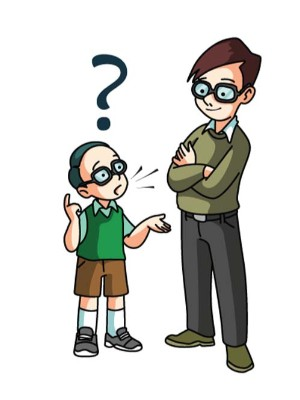
\includegraphics[width=0.4\columnwidth,trim=0 0 0 -3]{figures/I11.jpg}\\
\hline
Targeted (I11T): What is the boy doing?\\
\hline
Untargeted (I11U): What is happening? \\
\hline
\end{tabular}
\end{center}
\caption{Item 11, for which the core event is roughly \textit{boy asking question}.}
\label{fig:ask-question}
\end{figure}

%%\begin{table}[h]
%%\begin{center}
%%\begin{tabular}{|r|p{0.7\columnwidth}|c|c|}
%%\hline
%%& Response & Targeted & Untargeted \\
%%\hline
%%\hline
%%1 & the boy is asking questions to the man & yes & yes \\
%%\hline
%%2 & the boy is questioning & yes & yes \\
%%\hline
%%3 & he is asking the question & yes & yes \\
%%\hline
%%4 & the boy is asking & no & no \\
%%\hline
%%5 & this young boy presents a question that confused him for so long to his father & yes & yes \\
%%\hline
%%6 & the boy is asking for a problem to his father & no & no \\
%%\hline
%%7 & the brother is listening to his younger brother's question maybe he will answer it for him. & no & yes \\
%%\hline
%%8 & the boy is looking for answers & no & no \\
%%\hline
%%9 & the boy is expressing confusion to the man & no & no \\
%%\hline
%%10 & the boy is asking his father an existential question & yes & yes \\
%%\hline
%%11 & he is asking the man where babies come from & no & no \\
%%\hline
%%12 & he's asking his dad for something & no & no \\
%%\hline
%%13 & he is asking the man something & yes? & yes? \\
%%\hline
%%14 & he's asking for an explanation & ? & ? \\
%%\hline
%%15 & the child is curious about something and the father is trying to help him understand & no & yes \\
%%\hline
%%16 & this young man has multiple questions for his parent & no & no \\
%%\hline
%%17 & the boy is asking his father for some advice & no & no \\
%%\hline
%%18 & the boy is telling his dad a riddle & no & no \\
%%\hline
%%19 & the boy wants to know the answer to his question & no & no \\
%%\hline
%%\end{tabular}
%%\end{center}
%%\caption{\feat{core event} annotations for the targeted and untargeted versions of Item 11.}
%%\label{tab:core-event-cases}
%%\end{table}
\subsection{Verifiability} \label{subsec:verifiability}

The verifiability feature primarily considers the following question: \textit{Exactly as written, is all information in the response verifiable (or reasonably inferred) based on the image?}

This feature is mainly concerned with identifying inaccurate information and unverifiable inferences. 

\subsubsection{Contextuality of verifiability} Annotation for the verifiability feature is contextual; it must consider the image presented in the item. 

\subsubsection{Reasonable inferences} Responses that contain reasonable inferences should be considered verifiable. For this feature, an inference that can be assumed to be true for an overwhelming majority of situations like the one depicted in the image should be taken as \textit{reasonable}. Inferences that posit a degree of information that cannot safely be assumed (i.e., a \textit{guess}) should not be considered reasonable and should be annotated \textit{no} for verifiability. For example, the image in Figure~\ref{fig:carry-groceries} depicts a boy carrying a bag of groceries alone. The first example infers that the destination for the boy and his groceries is \textit{home}. This is taken as a reasonable inference because a person carrying a bag of groceries is almost certainly taking the groceries home. The second example describes the boy's action as \textit{helping carry} the groceries. This is also taken as a reasonable inference, because the small boy is very unlikely to be doing his own grocery shopping. The third example states that the boy is \textit{helping his mother} carry the groceries. Annotators should give this a \textit{no} for verifiability because the inference posits an unnecessary and unknowable level of detail; \textit{mother} is a fair guess here, but it is indeed a guess. Annotators must use their own best judgment in distinguishing between guesses and reasonable inferences.

\subsubsection{Subject and object variation} Because verifiability focuses on the truthfulness of information presented in responses, there are few restrictions regarding subjects for this feature. Even for targeted items, responses that omit or change the supplied subject may nonetheless be considered verifiable. Even responses that ignore the question entirely but present information that is verifiably true based on the image should be accepted. For this feature, participants are free to refer to subjects (and other entities) in the images as they wish, so long as they do so accurately and clearly. Responses to a targeted item that asks about \textit{the girl}, for example, may refer instead to \textit{the lady}, \textit{the young woman}, \textit{the short girl}, etc.; if the annotator believes such references are accurate, the responses should be annotated \textit{yes} for verifiability.

Many responses incorrectly describe a singular subject as plural or vice versa. In cases where the subject's number is clearly incorrect or too ambiguous to discern, the response should be annotated \textit{no} for verifiability. Some responses may indicate an incorrect number but still contain enough evidence that the correct number is intended, as in \textit{The two little kid are playing.} Given the \textit{two} and \textit{are}, this response should annotated \textit{yes}, despite the fact that \textit{kid} should be \textit{kids}. Annotators should use their best judgment in such cases.

With regard to objects, annotators should use their best judgment to determine if similar changes in number are acceptable. For example, a hunter shown shooting a single bird might nonetheless reasonably be described as \textit{hunting birds} or \textit{fowl}, but a salesman shown handing car keys to a lone female customer would not be reasonably described as \textit{selling a car to women} or \textit{selling cars to women}.

\begin{figure}[h]
\begin{center}
\begin{tabular}{|p{0.5\columnwidth}|p{0.3\columnwidth}|}
\hline
\multicolumn{2}{|c|}{
\includegraphics[width=0.4\columnwidth,trim=0 0 0 -3]{figures/I06.jpg}}\\
\hline
\textbf{Response} & \textbf{Acceptable inference?}\\
\hline
1. He's taking the groceries home. & yes \\
\hline
2. He's helping carry groceries. & yes \\
\hline
3. He's helping his mother carry groceries. & no \\
\hline
\end{tabular}{}
\end{center}
\caption{Example inference judgments (\textit{verifiability}) for \textit{What is the boy doing?}}
\label{fig:carry-groceries}
\end{figure}

\subsubsection{Language problems} Responses that are unintelligible should be annotated \textit{no} for verifiability; if the information in the response cannot be clearly understood, then it cannot be verified. However, grammar and spelling problems do not automatically result in a \textit{no} for verifiability. Responses that contain errors but remain reasonably clear and interpretable should be judged for verifiability like any other response.

\subsubsection{Incomplete responses} Responses that do not present a complete proposition should be annotated \textit{no} for verifiability. For example, untargeted responses that contain only a verb or verb phrase should be annotated \textit{no} for verifiability because they cannot be verified if the subject of the verb is unknown.

\subsubsection{Alternative interpretations} Although every effort was made to produce unambiguous PDT images, reasonable alternative interpretations are seen among the responses for some items. For example, Figure~\ref{fig:deliver-package} shows a woman seated behind a desk and a uniformed man standing across from her holding a package. Most participants interpret the scene as the man delivering a package to the woman. However, a small number of participants interpret this scene as a man picking up a package from the woman -- a reasonable alternative. Such reasonable alternatives should be annotated \textit{yes} for verifiability. Annotators should use their own in judgement in annotating responses that contain variations in interpretation.

\begin{figure}[h]
\begin{center}
\begin{tabular}{|c|}
\hline
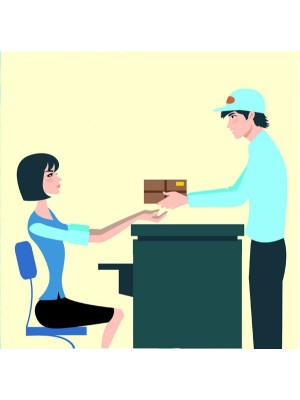
\includegraphics[width=0.4\columnwidth,trim=0 0 0 -3]{figures/I03.jpg}\\
\hline
Targeted (I03T): What is the man doing?\\
\hline
Untargeted (I03U): What is happening? \\
\hline
\end{tabular}
\end{center}
%\caption{Item 3, for which the core event is roughly \textit{man delivering a package}.}
\caption{Item 3, in the targeted and untargeted versions.}
\label{fig:deliver-package}
\end{figure}

\subsubsection{Responses in the form of a question} \label{subsubsec:verif-question} A small number of responses among the data take the form of a question. In general, such responses are not considered verifiable. For the verifiability feature, the content of the question is not taken as an assertion of facts and cannot be compared against the facts of the image. 

\subsubsection{Modality} Modality in a response can impact the verifiability. For annotation purposes, a sentence is \textit{modal} if it conveys the speaker's belief about the possibility of that sentence, using a modal verb (\textit{may, should,} etc.), or a modal adverb (\textit{maybe, perhaps,} etc.). (This is known as epistemic modality, because it involves the speaker's belief about the facts of the world.)

In a response where modality allows for doubt about the facts, the modal portions should be ignored, and the remainder of the response should be annotated for verifiability. For example, \textit{The man is smiling as he hands the woman a package, maybe he likes her} would still be annotated \textit{yes} for verifiability, because removing the modal portion (\textit{maybe he likes her}) leaves a verifiable statement based on the image (\textit{The man is smiling as he hands the woman a package}).

If, after removing the modal portions, a response is not verifiable, it should be annotated as \textit{no} for this feature. For example, in \textit{Perhaps the boy is asking a question}, the modal adverb has scope over the entire sentence, so removing the modal portion would leave no verifiable information.

\subsubsection{Unverifiable inferences} Responses containing unverifiable inferences are common among the data. Unverifiable inferences that embellish a response with unnecessary detail should result in a \textit{no} annotation for the response. For example, consider the item in Figure~\ref{fig:eat-pizza}, which shows a boy eating a slice of pizza. Some responses to this item refer to the pizza as \textit{sausage}, \textit{pepperoni} or \textit{cheese} pizza, and the image is ambiguous enough that one might argue for any of these descriptions. However, as these inferences cannot be confidently verified and they merely contribute detail, they should be annotated \textit{no} for verifiability.

Similarly, some creative responses assign names or other unknowable descriptors to persons in the PDT images. Such responses should be annotated \textit{no} for verifiability.

Some unverifiable inferences are arguably unavoidable based on the PDT item. For example, Figure~\ref{fig:ask-question} depicts a male child speaking to a male adult. Few participants could be expected to describe these figures as \textit{a male child} and \textit{a male adult} or something similarly unnatural. Instead, the image lends itself to reasonable inferences that describe the figures based on a relationship: a father and son, a big brother and little brother, or a student and teacher would all be reasonable and practically unavoidable inferences. 

Responses may contain other ``creative'' inferences, like \textit{He is asking the man where babies come from} (Figure~\ref{fig:ask-question}). This information is not verifiable, so the response is annotated \textit{no} for this feature.

\paragraph{Participant opinions} For annotation purposes, unverifiable information also includes statements that seem to derive only from the opinion of the participant, and not from the content of the image. To illustrate, consider Figure~\ref{fig:eat-pizza}, which depicts a boy eating a slice of pizza. In the first example response, \textit{He's eating a slice of delicious pizza}, the word \textit{delicious} is an expression of opinion, but based on the pleased expression on the boy's face, we can consider this reasonable and not solely dependent on the participant's opinion.

In the second example response, \textit{He's eating pizza, yuck}, the word \textit{yuck} can only be explained as the respondent's judgement about pizza, because there is nothing in the image to indicate that the pizza is \textit{yucky} or undesirable. 

\subsubsection{Irrelevant information} 
A less common problem to be considered under this feature is the presentation of irrelevant information. A response should be annotated \textit{no} for verifiability if it contains mostly irrelevant information, given the item. In Figure~\ref{fig:eat-pizza}, the third response, \textit{He will get fat eating pizza}, should be annotated \textit{no} because the event described is not relevant based on the PDT image and question.


\subsection{Answerhood} \label{subsec:answerhood}

The answerhood feature primarily considers the following question: \textit{Exactly as written, does the response make an attempt to answer the specific question asked?}

\subsubsection{Contextuality of answerhood} Annotation for the answerhood feature is contextual; it must consider the question presented in the item. The image is mostly irrelevant and is only used for targeted items to confirm that when a response replaces the subject with a pronoun, an appropriate pronoun is used.

\subsubsection{Defining \feat{answerhood}} As noted above, responses should address the specific question in the prompt. In other words, the response must answer the exact question given; merely answering a \textit{similar} or \textit{related} question is not adequate. Responses should make a positive assertion; responses that merely point out a negative fact are not acceptable (e.g., \textit{The boy is not wearing a helmet}.) In general, because all of the PDT questions use a present progressive verb, responses should either use a present progressive verb \textit{or} indicate an imminent action; see Section~\ref{subsubsection:answerhood-verbs}. Figure~\ref{fig:answerhood-examples} presents a number of example responses and answerhood annotations. 


\begin{figure}[h!]
\begin{center}
\begin{tabular}{|r|l|c|l|}
\hline
\multicolumn{4}{|c|}{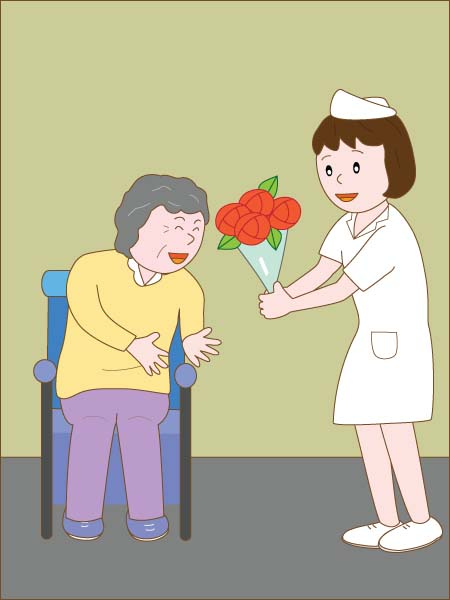
\includegraphics[width=0.4\columnwidth,trim=-4 0 -4 -4]{figures/ex01.jpg}}\\
\hline
& \textbf{Response} & \textbf{An.} & \textbf{Appropriate question} \\
\hline
1 & Giving a patient flowers. & yes & (prompt) \\
\hline
2 & She's giving flowers to a patient. & yes & (prompt) \\
\hline
3 & The nurse is giving away flowers. & yes & (prompt) \\
\hline
4 & A nurse is giving away flowers. & no & What is happening? \\
\hline
5 & A young nurse is giving away flowers. & no & What is happening? \\
\hline
6 & The woman is giving the patient flowers. & no & What is the woman doing? \\
\hline
7 & The nurse is happy. & no & How is the nurse? \\
\hline
8 & The nurse is smiling. & yes & (prompt) \\
\hline
9 & The nurse gives flowers away. & no & What does the nurse do? \\
\hline
10 & The nurse gave the patient roses. & no & What did the nurse do? \\
\hline
11 & The young nurse is giving out flowers. & no & What is the young nurse doing? \\
\hline
12 & The smiling nurse is giving away roses. & no & What is the smiling nurse doing? \\
\hline
13 & This nurse is giving away flowers. & no & What is this nurse doing? \\
\hline
14 & That nurse is giving her patient flowers. & no & What is that nurse doing? \\
\hline
15 & Nurse is giving away flowers. & no & What is Nurse doing? \\
\hline
16 & The patient is receiving roses from the nurse. & no & What is the patient doing?\\
\hline
%17 & The nurse is about to give the woman roses. & no & What is the nurse about to do? \\
%\hline
\end{tabular}
\end{center}
\caption{Example responses to targeted Item 2 (\textit{What is the nurse doing?}) and their answerhood annotations (\textit{An}). A particular response could be appropriate for multiple questions, but a likely example is given for each.}
\label{fig:answerhood-examples}
\end{figure}
\clearpage


\subsubsection{Accuracy} Answerhood should be annotated without regard to the accuracy of the response. Consider Figure~\ref{fig:eat-pizza} for example. The targeted version asks \textit{What is the boy doing?}; the response \textit{He's eating a sandwich} should be annotated \textit{yes} because it does attempt to answer the question, even though the boy is clearly eating pizza. Moreover, \textit{The boy is riding a bicycle} would also be annotated \textit{yes}, despite the fact that no bicycle appears. The accuracy of the response is accounted for with the core event and verifiability features.

\subsubsection{Targeted vs. untargeted items} The answerhood feature, like \feat{core event}, is dependent on the differences in the targeted and untargeted versions of the items. In other words, a sentence that may receive a \textit{no} annotation as a targeted response could receive a \textit{yes} annotation as an untargeted response. (The opposite should not be possible, as the targeted version of an item always asks a more specific question than its untargeted counterpart.) For example, consider Figure~\ref{fig:deliver-package} and the targeted and untargeted questions: \textit{What is the man doing?} and \textit{What is happening?} The response \textit{The man is delivering a package} would be annotated \textit{yes} for answerhood for either version, while \textit{The woman is receiving a package} would be annotated \textit{yes} only for the untargeted version.

%\subsubsection{Common answerhood concerns}

\subsubsection{Verb forms}
\label{subsubsection:answerhood-verbs}
The PDT items ask what \textit{is happening} or what a particular figure in the image \textit{is doing}, and these present progressive verb forms limit the range of acceptable responses. For the purposes of answerhood, acceptable responses should either employ a progressive verb form,  indicate imminent action, or present an appropriate event. These forms and related considerations are explained below.

\paragraph{Progressive verbs} The majority of responses use a dynamic verb in the progressive form. Dynamic verbs are appropriate for responses because they describe an event or action that happens and typically has a beginning and end. Dynamic verbs often take the (present) progressive form (\textit{(is) eating}, \textit{(is) dancing}). This is in contrast with stative verbs, which are inappropriate for this task as they describe a state or condition. Stative verbs cannot be used in the progressive form (with rare and arguably non-stative exceptions). Roughly speaking, stative verbs can be categorized as verbs of cognition (\textit{Susan knows karate}; \textit{Sabrina believes in the team}) and verbs of relation (\textit{Josh resembles his father}). Responses that rely on a stative verb should be annotated \textit{no} for answerhood. These responses (and any others) that simply describe a state of affairs in the image should be annotated \textit{no}, because they do not directly answer the question. For example, \textit{The boy loves pizza}, a response to Item 2 (Figure~\ref{fig:eat-pizza}) is annotated \textit{no} for answerhood, because it does not directly answer the question. Likewise, \textit{The nurse seems happy}, shown in Figure~\ref{fig:answerhood-examples}, should receive a \textit{no} annotation (for both the targeted and untargeted versions) because it describes a state depicted in the image but does not directly answer the question of what the nurse is \textit{doing}.

Although most responses use a present progressive verb (e.g., \textit{He \textbf{is eating} pizza}), responses using the simple present form of a verb (\textit{He eats pizza}) are also common among the data. This form is commonly used to describe general truths or habitual actions, like \textit{The horse eats grass} or \textit{The river flows east}. Responses that use the simple present should be annotated \textit{no} for answerhood. In most situations, in English the simple present would not be used to describe the actions in the PDT items, and particularly not in response to the present progressive questions in the PDT.

With the exception of \textit{event} responses (see Section~\ref{subsubsection:answerhood-events}) and \textit{imminent action} responses (see Section~\ref{subsubsection:answerhood-imminent}), responses that lack a progressive verb should be annotated \textit{no}, even if this is the only problem with the response. For example, \textit{The boy is hold a pizza} and \textit{The boy seems to eat pizza} would both be annotated \textit{no}. The mere appearance of a progressive form verb in a response does not automatically satisfy the answerhood feature, however. The necessary progressive verb must appear in a linguistic context that indicates that the verb directly responds to the question. For \textit{What is the dog doing?}, for example, the response \textit{The dog likes to chase the running cat} contains a progressive verb form, but not in a context that satisfies the answerhood feature.

Responses that omit a \textit{be} verb but include a progressive verb form in an otherwise appropriate context (e.g., \textit{The boy holding a pizza}) should generally be annotated \textit{yes} for answerhood. (The grammatical concerns are covered with the grammaticality feature.)

For handling misspelled verbs, see Section~\ref{para:answerhood-misspellings}

\subsubsection{Events and activities}
\label{subsubsection:answerhood-events} In some cases, a noun phrase may be an adequate and natural response to the PDT questions. For targeted items (\textit{What is the X doing?}), a response in the form of a noun or noun phrase that can be \textit{done} should be accepted. For example, \textit{gymnastics}, \textit{origami} and \textit{the laundry} are acceptable in response to \textit{What is the woman doing?}. Likewise, for untargeted items, a response in the form of a noun or noun phrase that can \textit{happen} should be accepted. For example, \textit{an interview}, \textit{a volleyball game} and \textit{a math class} are acceptable responses to \textit{What is happening?}.

For targeted and untargeted items, such event and activity responses should be properly formed as a grammatical response to the question, with any necessary determiners or articles. Grammar is not strictly considered for answerhood, but because these responses tend to be very short, proper form is used to differentiate between low-effort responses and those that appear to offer a thoughtful answer to the question. Such low-effort responses may simply describe some element of the image without considering the question. For example, \textit{a baseball game} should be accepted in response to the question \textit{What is happening?}, but \textit{baseball} and \textit{baseball game} should not.

\subsubsection{Imminent actions}
\label{subsubsection:answerhood-imminent}
Some responses describe the item in terms of an imminent action rather than a progressive action, e.g., \textit{The boy is about to eat the pizza}. Such imminent action responses are common among the responses from both native and non-native speakers. Some items elicit more of this type of response than others; Figure~\ref{fig:eat-pizza}, for example, shows a boy holding a slice of pizza near his mouth. Perhaps because the \textit{eating} action has not yet begun here, many responses indicate this as an imminent action rather than a progressive action. In general, responses that describe the subject's state in relation to an imminent action should be accepted, provided they otherwise fulfill the requirements for answerhood. However, responses that use a future aspect to describe the actions (e.g., \textit{The boy will eat the pizza}) do \textit{not} meet the requirements for answerhood.

Some responses do use a progressive form to indicate an imminent action, such as \textit{The boy is fixin' to eat the pizza} and \textit{The doctor is preparing to treat the patient}. Such responses should be annotated \textit{yes}, and annotators should be flexible in accepting variations and informal forms; for example, \textit{preparing, fixin', fixin}, and \textit{gonna} are all acceptable here.

In general, responses that describe the subject's state in relation to an imminent action are acceptable, with or without a progressive form. This includes responses that use these phrases (or others like them) followed by an action: \textit{is ready to, is getting ready to, is preparing to, is fixing to, is about to, is gonna}, etc. In the case of \textit{ready to} and \textit{about to}, because these expressions lack an actual verb, they must be preceded by a copular verb (\textit{is, seems}, etc.), which cannot be dropped. Likewise, the subject cannot be dropped. For example, \textit{preparing to eat the pizza} is acceptable in response to the question, \textit{What is the boy doing?}, but \textit{about to eat the pizza} is not acceptable.


\paragraph{Targeted subject variations and pronouns}
All targeted questions take the form of \textit{What is the X doing?}. Responses should use the same subject provided in the question, or an appropriate pronoun. This subject should be in the subject position of the response; if the response contains only a predicate, the subject of the question should be understood as the subject of the response. Responses should not alter the subject in any way, or move it from the subject position (as in passivization). This is in keeping with the requirement to answer the question exactly as it is asked. Several relevant examples are presented in Figure~\ref{fig:answerhood-examples}.

To put this concisely, responses to targeted items must either repeat the subject exactly as presented in the question, or use an appropriate pronoun, or drop the subject so that it is understood from the question. To clarify, the subject should not be altered in terms of definiteness, number, specificity, role or any other characteristic. Such responses add context to the question, and in order to evaluate answerhood, this new information would need to verified to ensure that the subject presented in the response is indeed the subject provided in the question. Verifying information for the sake of answerhood adds noise and complication, so verifiability is left to its own feature. For answerhood purposes, \textit{a nurse} is not the same as \textit{the nurse}. Likewise, neither \textit{nurse}, \textit{the young nurse}, \textit{the blond nurse}, \textit{the nurse who is standing}, or \textit{this nurse} is the same as \textit{the nurse}. Additionally, a targeted subject should not be expanded to include other persons or entities; in response to \textit{What is the man doing?}, \textit{The man is greeting the woman} is acceptable, while \textit{The man and woman are saying hello} is not.

Regarding pronouns, all humans presented in the PDT images are clearly male or female, and any targeted response that replaces the subject with a pronoun should use a pronoun that matches the subject's gender. Exceptions may be made for babies and animals portrayed in the PDT; the gender is not evident, and any third person singular pronoun is acceptable. For many items, the gender of the subject is clear from the question (\textit{What is the man/woman/boy/girl doing?}). Some items present a human subject in non-gendered terms, however, such as \textit{the nurse}, \textit{the teacher} and \textit{the doctor}. In these cases, annotators should check the image to ensure that appropriate gender pronouns are used. Pronouns should also match the subject in number, and all subjects in the PDT are singular. When a response presents a subject with a non-matching pronoun, annotators should mark this as \textit{no} for answerhood, because it is not possible to know if the response was indeed an attempt to answer the question asked. 

\paragraph{Misspellings}
\label{para:answerhood-misspellings}
The answerhood feature addresses whether or not a response \textit{makes an attempt} to answer the PDT question, so misspellings do not automatically result in a \textit{no} annotation. 

Annotators should be strict in handling misspelled subjects for targeted items. The subject is provided on screen for the participant, so misspellings should be avoidable. Only misspellings that are very clearly typos should be accepted here, such as \textit{t.he girl}. Misspellings that change the subject or leave it ambiguous in any way should be rejected. Pronouns must be properly spelled, but pronoun contractions that simply omit or misuse an apostrophe (e.g., \textit{Its} for \textit{It is}) should be accepted.

Verbs, even when misspelled, should appear to have the appropriate form (i.e., progressive). Annotators should be lenient with regard to misspelled verbs when a response appears to attempt to answer the question, even if the intended verb is not obvious. For example, \textit{The boy is steeaching his arms in bed} should be accepted, despite the badly misspelled attempt at \textit{stretching}.

When other elements of a response are misspelled, annotators should be lenient. The key consideration should be whether or not the response attempts to answer the question.

\subsection{Interpretability} \label{subsec:interpretability}
The interpretability feature primarily considers the following question: \textit{Exactly as written, is the response interpretable enough to evoke a clear image?} 

\subsubsection{Semi-contextuality of interpretability} \label{subsubsec:semicontext-interp} This feature is largely non-contextual, but because the task asks participants about events, responses must convey a proposition. In other words, a response must be interpretable as an event, or as a statement about the state of affairs in the image. Annotators may find it useful to view the PDT image, but interpretability should be judged without regard to its contents; to meet the criteria for this feature, a response should evoke \textit{an image}, regardless of how similar that image is to \textit{the image} in the PDT.

For targeted items only, when the subject of the response is omitted, it should generally be understood to be the same subject given in the targeted question. (This is not appropriate for \textit{all} responses that lack a subject, and annotators should use their judgment to decide if the respondent intended the subject to be understood.) For example, \textit{eating pizza} should be annotated as interpretable (according to the criteria below) as a response to the targeted question, \textit{What is the boy doing?}

In contrast, for the untargeted question (\textit{What is happening?}), a response like \textit{eating pizza} would not be interpretable, because a reader could not confidently conjure an image of the subject. (See Section~\ref{para:interp-incomplete} for more discussion of incomplete sentences.)

\subsubsection{Defining \feat{interpretability}} The interpretability feature is concerned with whether or not a response can be adequately understood and visualized. Because a response is based on an image, its interpretation should evoke a concrete image. A response should be considered interpretable if it A) includes any arguments that are syntactically required by the verb, and B) provides enough semantic content to derive a reasonably specific, unambiguous illustration.

\paragraph{Verb arguments} \label{para:interp-arguments} For this first requirement, \textit{A man is delivering a package to a woman} is interpretable. \textit{Delivering} is used as a ditransitive verb here, and all syntactically required arguments are specified; the sentence has a subject, direct object and indirect object. \textit{The man is delivering a package} should also be considered interpretable. This sentence does not include an indirect object, but in this transitive use of \textit{deliver}, the syntax does not require one. However, \textit{A man is delivering} is not interpretable, because the verb \textit{deliver} is missing one or more syntactically necessary arguments. This consideration requires a grammaticality judgment on the part of annotators. Annotators may have differing judgments with regard to the arguments required by given verbs; this is expected. Native speakers would likely agree that \textit{The man is cooking} is grammatical as is (without an object), and that \textit{The girl is telling} is not grammatical, because it requires an object (or more context). However, native speakers may disagree on the grammaticality of sentences like \textit{The boy is washing} or \textit{The woman is buying}.

\paragraph{Content and composition} Interpretable responses are statements that could be illustrated with a canonical composition, without the need to infer any critical elements. Responses that provide only a broad description are likely to fail this criterion. A sentence like \textit{The man is working} is not specific enough to evoke a clear image. An illustrator could show a man picking fruit, building a bridge, typing at a computer, etc., so long as the image contained a man doing some kind of work. A significant amount of information concerning the action in the image would need to be inferred.

Likewise, a sentence that uses vague references (\textit{someone/something}, unspecified \textit{it}, etc.) for essential elements or simply leaves them out is not interpretable. Such a response could not be illustrated as a canonical, representational painting, because some essential elements would have to be guessed or inferred. The response could, however, be represented as an abstract painting. 

It may be helpful for annotators to think of this as ``The Norman Rockwell Rule.'' That is, \textit{Would Norman Rockwell illustrate this response?} Straightforward composition and a clear representational style are hallmarks of Rockwell's paintings. A response like \textit{The man is delivering a package to a woman} fits this style of illustration. \textit{A man is delivering a package} also fulfills the Rockwell Rule, because a painting of a delivery man leaving a package in a mailbox or on a doorstep could easily be imagined as a Rockwell painting. (Annotators should keep in mind that interpretability annotation should not be influenced by the PDT image and the image evoked by the response is not judged here for how well it matches the actual PDT image.) For a response like \textit{Someone is delivering things to a woman}, a Rockwell painting simply would not fit; both the deliverer and the thing being delivered would have to be out of frame, obscured, somehow abstracted, or purely guessed at. Annotators should rely on their own judgment when considering these content and composition concerns.

\subsubsection{Common interpretability concerns}

\paragraph{Grammar and spelling} \label{para:interp-grammar} Grammar and spelling problems do not automatically result in a \textit{no} here; these concerns are covered by the grammaticality feature. Major or multiple grammar or spelling problems are likely to result in an uninterpretable sentence, but minor grammar or spelling problems may leave a sentence's interpretation intact. Annotators will vary in judging the severity of such problems, but in general, an annotator should mark a response as \textit{yes} for interpretability only when he or she can be reasonably confident in the intended meaning. In other words, a grammar or spelling problem that could be corrected in multiple ways to result in multiple reasonable corrected sentences should be marked \textit{no} for interpretability. As a reminder, for this feature, responses should be judged blindly, without influence from the image or previously seen responses.

For example, \textit{The boy is danceing} contains a spelling error, but a reader can be quite confident that the intended meaning is \textit{dancing}. \textit{The boy is dacing}, however, would likely be judged uninterpretable, because without more context, the error has numerous plausible candidates for correction -- \textit{racing, pacing, daring}, etc.

Responses that contain contradictory information should generally be marked \textit{no} for interpretability, but annotators should use their own discretion in handling these cases. Such problems often take the form of a noun phrase containing disagreement. For example, in \textit{The man is giving the package to a women}, it is impossible to determine if the indirect object would be illustrated as one woman or multiple women. If an annotator feels confident that other information in the response disambiguates the intended meaning, the annotator may rate the response \textit{yes} for interpretability. For example, in \textit{A young girls feeds a tasty carrot to her pony}, the determiner, the verb form and the later singular pronoun all indicate that \textit{girls} should be singular here.

Annotators should be lenient with subject-verb disagreement, unless they feel that such disagreement derails the interpretation of the response. For example, \textit{The children is playing ball} is unambiguous, despite the error.

\paragraph{Incomplete sentences} \label{para:interp-incomplete} Incomplete sentences should be annotated \textit{yes} for interpretability, so long as they fulfill the requirements explained above.

In general, responses may rely on information understood from the question. This means that for targeted items, where the question is of the form \textit{What is X doing?}, \textit{X is} may be understood for responses like \textit{washing the car} or \textit{jogging}. For certain responses, like \textit{the laundry} or \textit{the foxtrot}, \textit{X is doing} can be understood instead. In these cases, note that the response must be an action or event that is commonly described as being \textit{done}; \textit{do the laundry} is common expression, while \textit{do the baseball game} is not. 

Untargeted responses may also rely on information understood from the question, \textit{What is happening?} In these cases, \textit{is happening} may be understood when appropriate. This means that noun phrases that can \textit{happen} as events may be judged as interpretable, provided they otherwise fulfill the requirements of the feature. Therefore, \textit{A fight between a cat and a dog} would probably be marked \textit{yes} for interpretability, because it can \textit{happen} and it contains adequate information about the event participants. However, \textit{A fight}, which can also \textit{happen}, would be marked \textit{no}, because it cannot be illustrated confidently without more information.

Also common among the data are noun phrases resulting from a sentence with an omitted copular verb (\textit{be}), such as \textit{A man delivering a package} (as opposed to \textit{A man \textbf{is} delivering a package}). An omitted copula generally does not affect comprehension, so such a response should be annotated \textit{yes} for interpretability, provided it meets the above requirements for this feature.

Other forms of incomplete sentences appear in the data. Annotators should use their best judgment for these, but keep in mind that it is difficult for incomplete sentences to satisfy the criteria, especially for untargeted items, where very little information can be understood from the question.

\paragraph{States and actions} \label{para:interp-question} The PDT is designed to elicit responses that describe an action; as a result, most responses contain an active verb. Some responses, however, describe a state of affairs in the image, such as \textit{The boy is wearing a green shirt} or \textit{The boy is ready to eat his pizza}. Responses that describe a state are nonetheless interpretable, so long as they fulfill the remaining criteria.

\paragraph{Questions and modals} \label{para:interp-question} A small number of responses among the data take the form of a question. Some of these responses nonetheless present an assertion. For example, \textit{Why is the baby crying?} indicates that \textit{the baby is crying}. This response should be annotated \textit{yes} for interpretability, because the assertion it contains meets the criteria for interpretability.

Some responses in the form of a question lack an assertion that can be judged for interpretability, e.g., \textit{Do you think the boy likes pizza?} Such responses are not interpretable.

Responses that use modality may be considered interpretable if the modality does not effect information crucial to producing a visual representation. For example, in \textit{The boy is eating so much pizza he may get fat}, it is stated as fact that a boy is eating pizza, so this could be visually represented. The modal part of this sentence contains unnecessary detail and could be ignored. In contrast, in \textit{The man may be proposing marriage to the woman} the modality has scope over the whole predicate, so this response should be marked \textit{no} for interpretability. (The man \textit{may} be proposing marriage to the woman, but there is no limit to the number of things he \textit{may} be doing.)

\paragraph{First and second person} All entities in the PDT items should be represented in the third person. Responses that use the first or second person to indicate a participant in the image should be considered uninterpretable. For example, \textit{A young man will mail a package for you} should be marked \textit{no}. 

\paragraph{Slang} Some responses contain what may be considered slang. Such responses are interpretable if they meet the other requirements for interpretability. For example, \textit{The boy is getting his groove on} would probably be taken to mean that the boy is dancing intensely and could thus be considered interpretable. A response that contains unclear or unknown slang should be considered uninterpretable. Annotators must rely on their own judgment regarding slang.

\paragraph{Impossible or unknowable information} All PDT items consist of a single image. They present information in a straightforward manner and are almost completely devoid of any text, signs or symbols. Thus all responses should present information that can be learned from such an image. Responses that present important information (not details) that could not be known from or represented with a single image should be marked \textit{no} for interpretability. For example, \textit{He is sending a box to a woman} could not be easily represented in a single image, as the man sending the box and the woman receiving the box would be in different locations. Moreover, the man and woman (and box) are arguably equally important arguments, so choosing whether to omit the subject or indirect object when illustrating the image would be problematic.

Responses that present an interpretable proposition but embellish it with unknowable details should be considered interpretable. (Note that concerns about unverifiable information are captured under the verifiability feature.) For example, \textit{As the man hands the package to the woman, their eyes meet and a passionate romance ensues} presents a simple, illustratable event -- a man handing a package to a woman, perhaps while making eye contact. The remaining details are unnecessary for assessing interpretability. Annotators must use their own judgment in such cases.


\subsection{Grammaticality} \label{subsec:grammaticality}
The grammaticality feature primarily considers the following question: \textit{Exactly as written, does the response convey a proposition and does it lack any grammar or spelling errors?}

\subsubsection{Non-contextuality of grammaticality} This feature considers only the response, regardless of the item or question. In other words, a response that is grammatical but  irrelevant given the specific item image and question should still be annotated as \textit{yes} for this feature.

However, grammaticality should be annotated within the bounds of the very general context of the task; the PDT elicits descriptions of common events, so responses should convey a proposition and be grammatical when interpreted accordingly.

Moreover, the item question may be taken into consideration when it is necessary for assessing the grammaticality of a particular response. Responses to targeted questions (\textit{What is the X doing}), for example, commonly drop the subject. Such responses can be grammatical; see Section~\ref{subsubsec:gram-incomplete-sentences}.

\subsubsection{Defining \feat{grammaticality}} For the current annotation purposes, a \textit{grammatical} response is one that is free from grammar errors or misspellings, and conveys a reasonable meaning (given the very general context of the task). Grammar errors come in many forms, including omitted words, out-of-place words, incorrect word forms, and syntactic disagreement, among others. This feature does not directly consider \textit{meaning}. However, the events depicted in the PDT images are all common, unsurprising events that might occur under normal circumstances, and a response that requires an unreasonable interpretation in order to be grammatical should be annotated \textit{no} for grammaticality. For example, \textit{The boy is dancing on music} is probably not grammatical without resorting to a fairly unusual interpretation -- perhaps involving a boy dancing on a floor covered with sheet music or vinyl records.

Annotators will need to make judgment calls, but should be lenient in judging grammaticality and the necessary interpretation of meaning. If there is a reasonable reading of the sentence under which it is grammatical (and has none of the specific grammaticality problems outlined below), it should be annotated as \textit{yes}. (Annotators should keep in mind that concerns other than grammar are likely to be captured under the annotation of other features.) For example, consider this response to the item in Figure~\ref{fig:dance}: \textit{A boy listens to music and dancing}. Given the image, one could point out that the meaning conveyed by the response is not the intended meaning (presumably \textit{A boy listens to music and (he) dances}), and thus argue that the response is ungrammatical. However, because the response is not ungrammatical without the item context, and it conveys an arguably reasonable meaning, such a response should be annotated \textit{yes}. This also commonly applies to responses that use an incorrect (but grammatical) pronoun. For example, \textit{The boy is talking to her brother}, in response to Figure~\ref{fig:ask-question} (where no female is pictured or otherwise indicated as a potential antecedent to \textit{her}), should be annotated \textit{yes} for grammaticality.

\subsubsection{Incomplete sentences} \label{subsubsec:gram-incomplete-sentences} Although the task asks participants to provide a complete sentence, incomplete sentences (which are mostly verb phrases among the data) may nonetheless be annotated as \textit{yes} for grammaticality, so long as the content of the response is indeed grammatical. For example, \textit{eating pizza} is an incomplete sentence but a grammatical response. This also applies to any one word responses, but as explained in Section~\ref{para:non-propositional}, a grammatical response should be interpretable as a proposition. For example, \textit{eating} should be considered a grammatical response, because it conveys some propositional meaning, but \textit{pizza} is not grammatical here because it does not indicate any action or event. Incomplete sentences are subject to all of the same grammaticality considerations as complete sentences.

\subsubsection{Punctuation and capitalization} Responses have been converted to all lowercase letters. Final punctuation has been removed from most responses. Annotators should ignore these concerns when annotating grammaticality. 

Sentence internal punctuation should be considered for this feature, but annotators should be lenient and keep in mind that many punctuation decisions may simply be a matter of style rather than grammar. Punctuation (or lack thereof) that results in ambiguity or leads the annotator to question the overall grammaticality of the sentence should result in a \textit{no} annotation for the response. Annotators should use their own best judgment in assessing such cases.

\subsubsection{Common grammaticality concerns}

\paragraph{Events and activities}
\label{para:gram-events} In some cases, a noun phrase may be an adequate and natural response to the PDT questions. For targeted items (\textit{What is the X doing?}), a response in the form of a noun or noun phrase that can be \textit{done} should be considered grammatical. For example, \textit{gymnastics}, \textit{origami} and \textit{the laundry} are acceptable in response to \textit{What is the woman doing?}. Likewise, for untargeted items, a response in the form of a noun or noun phrase that can \textit{happen} should be accepted. For example, \textit{an interview}, \textit{a volleyball game} and \textit{a math class} are acceptable responses to \textit{What is happening?}.

For targeted and untargeted items, such event and activity responses should be properly formed as a grammatical response to the question, with any necessary determiners or articles. For example, \textit{a baseball game} should be accepted in response to the question \textit{What is happening?}, but \textit{baseball} and \textit{baseball game} should not.

\paragraph{Non-propositional responses} \label{para:non-propositional} A response that lacks a grammatical interpretation \textit{as a proposition} should be annotated \textit{no} for grammaticality. A proposition typically requires a verb and a subject; for the current task, a response may be judged as grammatical if it lacks a subject so long as it indicates an action or event. Non-propositional responses do not fit the general context of the task. These responses typically lack a verb and some appear to be well-formed noun phrases, such as \textit{A boy with pizza}.

\paragraph{Bare nouns} A bare noun that is missing a determiner should result in a \textit{no} for grammaticality. Examples include \textit{Boy is eating pizza} and \textit{A man is delivering package}.

\paragraph{Missing \textit{be} verbs} Common among the data are responses that omit a necessary copula (or \textit{be} verb). These often result in what could be interpreted as well-formed noun clauses, such as \textit{A little boy eating pizza}. If, as in this case (and most others), one can reasonably assume that the apparent noun clause is an ungrammatical expression of a copular sentence (\textit{A little boy \textbf{is} eating pizza}), the response should be annotated \textit{no} for grammaticality. 

Note that incomplete sentences that omit the subject may also omit a \textit{be} verb. In other words, while \textit{A little boy eating pizza} should be annotated \textit{no} for grammaticality, simply \textit{eating pizza} may be annotated as \textit{yes} if appropriate. (See Section~\ref{subsubsec:gram-incomplete-sentences}.)

\paragraph{Misspellings} Misspellings generally result in a \textit{no} for grammaticality. Misspellings sometimes result in real but unintended words, so it is not always clear if a word is in fact a misspelling. A response containing a suspected real word misspelling should be annotated \textit{no} for grammaticality only if it results in a grammar error.

Some responses use proper names for persons, places or objects in the images. When a proper noun appears to be misspelled, annotators should be less strict. If the proper noun is reasonably interpretable, the response should still be annotated \textit{yes}, provided it has no other disqualifying problems. Annotators should use their own judgment in assessing such cases.

\clearpage

\subsection{Example items}

\begin{figure}[h]
\begin{center}
\begin{tabular}{|c|c|}
\hline

\includegraphics[width=0.35\columnwidth,trim=0 0 0 -3]{figures/I01.jpg} & 
\includegraphics[width=0.35\columnwidth,trim=0 0 0 -3]{figures/I02.jpg}\\
\hline
I01T: What is the boy doing? & I02T: What is the boy doing? \\
\hline
\hline
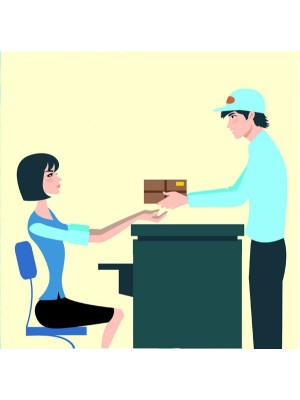
\includegraphics[width=0.35\columnwidth,trim=0 0 0 -3]{figures/I03.jpg} & 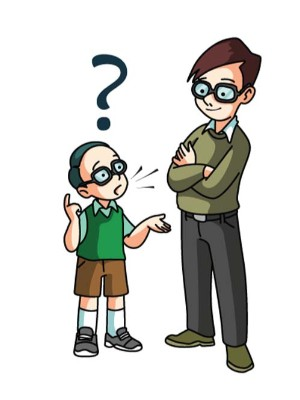
\includegraphics[width=0.35\columnwidth,trim=0 0 0 -3]{figures/I11.jpg}\\
\hline
I03T: What is the man doing? & I11T: What is the boy doing? \\
\hline
\end{tabular}
\end{center}
\caption{Example items, including \textit{targeted} questions. The question for all \textit{untargeted} items is \textit{What is happening?}}
\label{fig:appendix1}
\end{figure}

\clearpage 

\bibliographystyle{plainnat}
\bibliography{mybib}

\end{document}



